% ======================================================================
% doc_body.tex -- the main document content.
%
% This template is for UNCG's PHY 419 (Advanced Lab) course,
% Assignment 1: Research Proposal.
%
% Adapted from the APS REVTeX 4.2 template in Overleaf on 2019-08-20.
%
% This file is part of the APS files in the REVTeX 4.2 distribution.
%     Version 4.2a of REVTeX, December 2014
%     Copyright (c) 2014 The American Physical Society.
%     See the REVTeX 4 README file for restrictions and more information.
%
% Using this requires BibTeX. Overleaf handles this automatically,
% **if** you have the right files in your project folder (*.bib),
% and you recompile both this document and the *.bib document after
% making changes to what's in *.bib.
%
% Note that the comment character "%" has been used to deactivate
% certain lines below, but keep the code in the file in case you want
% to reactivate them at some point.% to reactivate them at some point.


%
% ======================================================================
\documentclass[%
reprint,
%superscriptaddress,
%groupedaddress,
%unsortedaddress,
%runinaddress,
%frontmatterverbose, 
%preprint,
%preprintnumbers,
%nofootinbib,
%nobibnotes,
%bibnotes,
amsmath,amssymb,
aps,
%pra,
%prb,
%rmp,
%prstab,
%prstper,
%floatfix,
]{revtex4-2}

\usepackage{graphicx}% Include figure files
\usepackage{dcolumn}% Align table columns on decimal point
\usepackage{bm}% bold math
\usepackage{hyperref}% enables hyperlinks in the PDF
\usepackage{xcolor}
\usepackage{graphicx}
\usepackage{dcolumn}
\usepackage{bm}
\usepackage{hyperref}
\usepackage{booktabs}
\usepackage[noabbrev]{cleveref}
\usepackage{algorithm}
\usepackage{algorithmic}

\binoppenalty=\maxdimen
\relpenalty=\maxdimen

\newcommand\todo[1]{\textcolor{red}{#1}}


\begin{document}
	
	\title{Resampling in Particle Filters - an Optimal Transport approach}% Force line breaks with \\
	
	\author{Adrien Corenflos} % Probably you, the student
	%\email{adrien.corenflos@gmail.com}
	%\affiliation{Quantitative Researcher, J.P. Morgan}
	\date{\today}% It is always \today, today,
	%  but any date may be explicitly specified
	
	\begin{abstract}
		We use recent advances in optimal transport to tackle the challenge of resampling in particle filters. In particular we propose one approximate differentiable scheme and two exact schemes to transform a weighted empirical distribution into a similar unweighted distribution. 
		\\
		
		Keywords: differentiable, resampling, particle filters, smc, optimal transport, divergence
	\end{abstract}
	

	
	\maketitle
	% ========================================================================
	
	\section{Introduction \& Previous works}
	
	Particle filters have emerged as a state of the art inference technique for non linear State Space Models.
	
	\todo{include description of Bootstrap filter}
	\label{algo:bootstrap}
	
	The resampling in \cref{algo:bootstrap} is included to fight degeneracy of the particles and some alternatives have been proposed to find an optimal re-indexing index $\sigma : \left\{ 1,\dots, N \right\} \to \left\{ 1,\dots, N \right\}$ (see \todo{include ref about different schemes}). This resampling step notoriously makes the particle filter non-differentiable with respect to their hyper-parameters as it creates a non-differentiable mapping , $(w_i, X_i) \mapsto (1/N, X_{\sigma(i)})$.

	Most of these approaches rely only on the weights $(w_i)_i$ to provide a probabilistic resampling variable $(\sigma_i)_i$ that verifies $\mathbb{E}[\sigma_i = i] = w_i$ (\todo{reference on coherence of resampling schemes}). These don't take into account the geometry of the space and create duplicates of particles.
	
	On the other hand some approaches have been tried that take into account the distance between the particles. The most similar work to our approach is \cite{reich2012nonparametric} where the author explicitly creates an optimal transport plan $T$ such that $\tilde{X} = N T X$ mapping from the weighted particles to the unweighted ones.
	
	The paper is organised as follows:
	
	\begin{enumerate}
		\item Approximate reweighting using optimal transport mapping and differentiability
		\item Exact reweighting using global divergence minimization
		\item Fast exact reweighting
		\item Particle filter examples (probably learn the parameters of Lorentz system in dimension 3, and track with known parameters in higher dim, using section 2 and 3)
	\end{enumerate}
		

	\section{Approximate reweighting using optimal transport mapping}
	\label{sec:approximate}
		\subsection{The algorithm}
		In \cite{reich2012nonparametric} the author defines the planning matrix $T \in \mathbb{R}^N$
		as the solution to the optimal transport problem:
		
		\begin{align*}
			T &= \text{argmin}{\sum_{i, j} T_{i,j}  d(X_i,X_j)} \, \text{with} \\
			\forall j, & \sum_i T_{i, j} = w_i \, \text{and} \, \forall i, \sum_j T_{i, j} = 1/N
		\end{align*}
		\\
	
		In practice the distance $d$ is chosen to be the euclidean distance or the Manhattan distance.
		However optimal transport calculation scales as $O(N^3)$, which makes the approach in \cite{reich2012nonparametric} unfeasible for cases where a large number of particles need to be used.

		Regularized optimal transport has emerged as way to solve such constraints \cite{cuturi2013sinkhorn} where the optimal transport problem is replaced with the following \todo{include definition of the optimisation problem}. An alternative formulation that we will use in the rest of this article is given by \cite{feydy2018interpolating}, \todo{copy the algorithm}. In their paper they moreover prove the differentiability of their scheme.
		We combine their approach and the one in \cite{reich2012nonparametric} to provide a differentiable rebalancing scheme:
		
		$$\tilde{X}_{\epsilon} = N T_{\epsilon}^t X$$ where $T$ is the solution of $L_{\epsilon}(w, X, \frac{1}{N}, X)$.
			
		
		We illustrate the behaviour of type of rebalancing in \cref{fig:rebalancing_map} \todo{The EMD in python POT doesn't work, need to raise an issue on the github, the "exact scheme" is sinkhorn with very small reg}, where $X \sim \sum_i w_i, \delta_{X_i}$, the $X_i$'s are i.i.d. $U([-2, 2])$ and $w_i \propto f(X_i)$ where $f$ is the pdf of a normal distribution $\mathcal{N}(\text{loc}=0.5, \text{scale}=1)$ and $N = 500$, i.e. $\frac{1}{N} = 0.002$ \label{def:example}
		
		In practice the resulting weighting $N T_{\epsilon} w$ will not be totally flat due to the fact that $T$ is an approximation: \cref{tab:transformedWeights} shows how the weights are distributed depending on the regularisation. Moreover, their value doesn't depend on the past. We will therefore set the value of $N T_{\epsilon} w \simeq 1/N$  to $\frac{1}{N}$ and its gradient w.r.t. $w$ and $X$ to $\mathbf{0}$ in the rest of the article.
		
		
		\begin{table}
			\begin{tabular}{lrrrr}
				\toprule
				$\bm{\epsilon}$ &        0.01 &       0.05 &       0.10 &       0.50 \\
				\midrule
					mean  &      1.995 &      1.998 &      1.998 &      2.001 \\
					std   &      0.152 &      0.099 &      0.089 &      0.049 \\
					quantile 10\%   &      1.801 &      1.874 &      1.875 &      1.919 \\
					median   &      2.009 &      2.020 &      2.023 &      2.015 \\
					quantile 90\%   &      2.197 &      2.106 &      2.096 &      2.050 \\
				\bottomrule
			\end{tabular}
			\label{tab:transformedWeights}
			\caption{distribution of rebalanced weights ($\times 100$0) as a function of epsilon}
		\end{table}
		
		
		\begin{figure}
			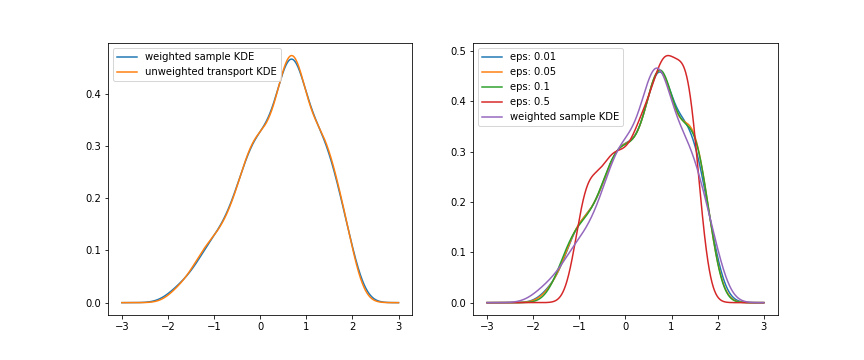
\includegraphics[width=\linewidth]{KDEIllustration}
			\caption{
				Guaussian KDE for different transport schemes
				left: exact transport scheme, right: regularized transport scheme for different values of $\epsilon$}
			\label{fig:rebalancing_map}
		\end{figure}	
	
		\subsection{Gradients}
			As discussed in \cite{feydy:hal-01827184} the gradients for $(w_i, X_i) \mapsto \alpha, \beta$ are readily available using the implicit function theorem. 
			Moreover the potentials and the transport matrix are linked via:

			\begin{align*}
				T_{\epsilon} &= \exp \tfrac{1}{\epsilon^2}[\alpha\oplus \beta - \text{C}] \cdot \alpha\otimes \beta \\
				~& \text{which in our case can be rewritten as:}\\
				T_{\epsilon} &= \frac{\exp{(\alpha^t + \beta -\frac{C^2}{2})}}{\epsilon^2} w^t / N
			\end{align*}

			where $C = d(X_i, X_j)_{1 \leq i, j\leq N}$ and the exponential has to be understood element-wise.
			
			This in turn means that the mapping $(w_i, X_i) \mapsto \tilde{X}_{\epsilon}$ is differentiable with gradient given by $\text{d}\tilde{X}_\epsilon = N \text{d}T_\epsilon X + N T_\epsilon \text{dX}$
		
			
			\todo{Some problems with the gradients coming from geomloss: they are only coded for the sake of differentiating the loss function, not the potentials. I'm chatting with Jean Feydy, I've patched by using eq (27) in \cite{feydy:interpolating} but need to check consistency formally}
				
			To illustrate the fact that our method works we compute the analytical gradient $ \frac{\partial }{\partial \text{loc}} \left( \tfrac{1}{N} \sum_{1 \leq i\leq N } w_i X_i \right)$ when $w$ and $X$ are given as in \cref{def:example} for different values of the locations and the scale. The analytical gradient is given by:
			
			$$ 
			\frac{1}{4} \int_{-2}^{2}\text{pdf}(x, loc, scale) x \frac{x-loc}{\text{scale}^2} dx
			$$
			
			Numerically the result is shown in tables \cref{tab:gradients}.
			
			
			\begin{table}
				\centering
				\begin{tabular}{lrrrrr}
					\toprule
					{} &     -0.5 &     -0.25 &      0 &      0.25 &      0.5 \\
					\midrule
					0.25 &  0.25 &  0.25 &  0.25 &  0.25 &  0.25 \\
					0.5 &  0.25 &  0.25 &  0.25 &  0.25 &  0.24 \\
					1 &  0.16 &  0.18 &  0.18 &  0.18 &  0.16 \\
					1.5 &  0.09 &  0.09 &  0.10 &  0.09 &  0.09 \\
					2 &  0.05 &  0.05 &  0.05 &  0.05 &  0.05 \\
					\bottomrule
				\end{tabular}
				\caption{Theoretical gradients, line: scale, column: location}
			\vfill

				\begin{tabular}{lrrrrr}
					\toprule
					&     -0.5 &     -0.25 &      0 &      0.25 &      0.5 \\
					\midrule
					0.25 &  0.05 &  0.12 &  0.15 &  0.12 &  0.04 \\
					0.5 &  0.14 &  0.23 &  0.26 &  0.25 &  0.16 \\
					1 &  0.12 &  0.17 &  0.19 &  0.17 &  0.114 \\
					1.5 &  0.05 &  0.05 &  0.05 &  0.05 &  0.05 \\
					2 &  0.02 &  0.02 &  0.02 &  0.02 &  0.02 \\
					\bottomrule
				\end{tabular}
				\caption{AutoDiff Gradients, line: scale, column: location}
				\label{tab:gradients}
			\end{table}
	

	\section{Exact reweighting using global divergence minimization}
	\label{sec:exact reweighting}
		While the scheme in \cref{sec:approximate} has the advantage of providing a gradient for the resampling schemes, it suffers from the inconvenient of approximating the reweighted sample through a linear mapping only. While this can be useful for cases where the latent space regular enough, some more complex cases may arise where a linear mapping doesn't suffice anymore. This is true in particular when most of the particles are degenerate and when the distribution is multimodal \todo{Don't know if that's a good example, need Arnaud}
		
		This is illustrated in \cref{fig:degenerate_map} where the example in \cref{sec:approximate} has been modified in the following way: out of 500 particles distributed uniformly between -2 and 2, 250 have been chosen randomly and their weight set to the normal pdf with mean 0.5 and scale 0.1 and the rest to the normal pdf with mean -1 and scale 0.1. This is equivalent to a NESS of 41. As expected the linear transportation doesn't provide a good approximation of the degenerate distribution.
		
		\begin{figure}
			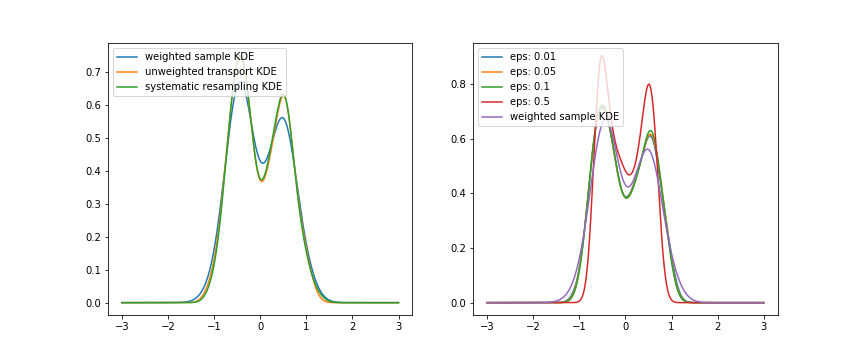
\includegraphics[width=\linewidth]{DegenerateTransport}
			\caption{
				Guaussian KDE for different transport schemes
				left: exact transport scheme and systematic resampling, right: regularized transport scheme for different values of $\epsilon$}
			\label{fig:degenerate_map}
		\end{figure}	
		
		To alleviate this issue we propose to modify the algorithm above by using an approach similar to \cite{genevay2017learning} and find unweighted $\tilde{X_epsilon}$ minimising a certain distance w.r.t. the degenerate sample $(w, X)$. As discussed in \cite{feydy:interpolating} the entropic bias induced by the regularisation term in regularised Optimal Transport results in concentrated distributions, which is the opposite of our goal. Following \cite{genevay2017learning} we therefore use the unbiased version of the Sinkhorn iterates: the Sinkhorn divergence. \todo{Include some background with feasibility \cite{feydy:interpolating} and proof of metrisation}.
		
		We therefore aim at minimising 
		
		\begin{align*} 
			S_\epsilon(\cdot)_{X, w} 
				&= OT_{\epsilon}\left(\frac 1 N, \cdot, w, X\right) \\
				&- 0.5 OT_\epsilon\left(\frac 1 N, \cdot, \frac 1 N, \cdot \right) \\ 
				&- 0.5 OT_\epsilon(w, X, w, X)
		\end{align*}
		
		This is done via a gradient descent leveraging Adam.
		
		\begin{figure}
			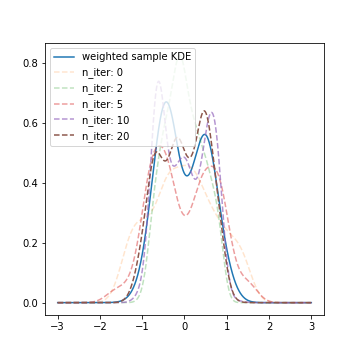
\includegraphics[width=\linewidth]{LearntDist}
			\caption{
				Guaussian KDE for learnt unweighted distribution.
				Convergence of the unweighted distribution to the weighted one as the number of epochs increases
				}
			\label{fig:learntResampling}
		\end{figure}	
		
		It converges but maybe not the best thing to do...
		
		
	\section{Fast exact reweighting}
	\label{sec:fast reweighting}
		\todo{I want to modify the scheme in \cref{sec:exact reweighting} by doing something similar:}
		
		Instead of going minimising the divergence by starting from the (1/N, X)
		
		\begin{align*} 
			S_\epsilon(\cdot)_{X, w} 
			=& OT_{\epsilon}\left(\frac 1 N, \cdot, w, X\right) \\
			&- 0.5 OT_\epsilon\left(\frac 1 N, \cdot, \frac 1 N, \cdot \right) \\ 
			&- 0.5 OT_\epsilon(w, X, w, X)algorithm
		\end{align*}
		
		It may be worth taking a lookahead approach: given a schedule $0 = t_1< t_i < t_N = 1$, we can successively minimise for $k = 1, ..., N-1$:
		$$X_{k+1} = \text{argmin}_z(S_\epsilon(X_k, w_k, z, w_{k+1})$$
		
		Where $w_{k} = t_k \frac 1 N + (1 - t_i)  w$ and $X_0 = X$ . If the step size is taken small enough, $X_k, w_k$ and $X_{k+1}, w_{k+1}$ will be close enough to allow for an immediate minimisation at every step.
					
		
		\begin{algorithm}
			\caption{Incremental learning}
			\label{alg:incremental}
			\begin{algorithmic}
				\STATE {\bfseries Input:} $x$, $w$, $t$, $N$, $\lambda$, $K$ \COMMENT{Number of gradient descent loops}, 
				\STATE {\bfseries Compute:} $w_i := t_i \frac 1 N + (1 - t_i)  w, i=1..N$
				\STATE Initialize $x_i = x$.
				\FOR{$i=1$ {\bfseries to} $N$}
					\STATE $y_k = x_i$
					\FOR{$k=1$ {\bfseries to} $K$}
						$y_k = y_k - \lambda \nabla_y S_\epsilon(S_\epsilon(x_i, w_i, y_k, w_{i+1})
				\ENDFOR
					\STATE x_i = y_k
				\ENDFOR
			\end{algorithmic}
		\end{algorithm}

	\bibliography{bib}
	\bibliographystyle{plain}



\end{document}

%%%%%% End of file doc_body.tex %%%%%%